%!TEX root = TQFTnotes.tex
%%%%%%%%%%%%%%%%%%%%%%%%%%%%%%
\chapter{PL manifolds, triangulations, and polygon decompositions}\label{c:PL}

In this chapter, we start building an alternative approach to the construction
of extended TQFTs. Instead of using Morse functions to decompose a cobordism
into a product of elementary cobordisms, we will use triangulations and similar
cell decompositions. This is naturally done in the category of piecewise-linear
(PL) manifolds; thus, in this chapter we will work with PL manifolds. We refer
the reader to \cite{rourke} for an overview of PL topology; another useful
reference is Lurie's lecture notes \cite{lurie-PL}.

%%%%%%%%%%%%%%%%%%%%
\section{Polyhedra and PL manifolds}\label{s:polyhedra-pl}
\begin{definition}
  A $k$-simplex $\si\subset \R^N$ is the convex hull of a set of $k+1$ points
  $x_0, x_1, \dots, x_k$ which are affinely independent, i.e., span an affine
  subspace of dimension $k$ in $\R^N$.

  A finite polyhedron is a subset $P\subset \R^N$ which can be presented as a
  finite union of simplices.
\end{definition}
Note that for a given polyhedron, there are many ways to present it as a union
of simplices. We will be mostly working with triangulations.

\begin{definition}\label{d:triangulation}\index{triangulation}
  A triangulation of a polyhedron $P\subset \R^N$ is a finite
  collection $S=\{\si_i\}$ of simplices such that $P=\bigcup_S \si_i$
  and
  \begin{enumerate}
    \item Any face of a simplex $\si\in S$ is again a simplex in $S$.
    \item The intersection of any two simplices from $S$ is a face of each of them.
  \end{enumerate}
\end{definition}
(Note that by ``face'', we mean a face of any codimension, not necessarily
 codimension 1).

\begin{theorem}\label{t:triangulation1}
  \par\noindent
  \begin{enumerate}
  \item
    Any finite polyhedron $P\subset \R^N$ admits a triangulation.
  \item
    Any two triangulations of a finite polyhedron $P$ admit a common
    subdivision: if $T_1,T_2$ are triangulations, then there exists a
    triangulation $T_3$ such that each simplex of $T_1$ is a union of simplices
    of $T_3$, and the same for $T_2$.
   \end{enumerate}
\end{theorem}
We refer the reader to \cite[Theorem 2.11, Addendum 2.12]{rourke} for
the proof.
\begin{definition}\index{piecewise linear!map}
  Let $P$ be a polyhedron. A function $f\colon P\to \R^m$ is called \emph{%
  piecewise linear} (PL) if it is continuous and there exists a triangulation of
  $P$ such that the restriction of $f$ to each simplex of the triangulation
  is linear.

  For polyhedra $P\subset \R^N$, $L\subset \R^m$, a map $f\colon P\to L$
  is piecewise linear if it is piecewise linear as a map $P\to \R^m$.
\end{definition}
It is easy to see that the composition of PL maps is again PL; thus, we get a
category of PL polyhedra.

\begin{remark}
  Above, we defined polyhedra as subsets of $\R^N$. Choosing a triangulation
  gives a combinatorial description of $P$: all we need to know is how many
  simplices there are of each dimension and which faces are glued together. One
  can define an \emph{abstract simplicial complex} $K$ as such combinatorial
  data (we skip the precise definition). Conversely, given an abstract
  simplicial complex, we can construct a polyhedron $P=|K|$ by gluing together
  simplices along the face maps and embedding this union of simplices in $\R^N$
  for sufficiently large $N$; moreover, such a polyhedron is unique up to PL
  isomorphism.
\end{remark}

\begin{definition}\label{d:PLmanifold}
  Let $M$ be a polyhedron. We will say that $M$ is a \emph{PL manifold}\index{PL
  manifold} of dimension $n$ if, for every point $x \in M$, there exists an open
  neighborhood $U \subset M$ containing $x$ and a piecewise linear homeomorphism
  $f\colon U \to U'$ where $U'$ is a neighborhood of 0 in $\R^n$.
\end{definition}
\begin{remark}
  If $M$ is a PL manifold, then its underlying topological space is
  automatically a topological manifold. The converse, however, is not true: it
  is possible to construct a polyhedron $P$ such that the underlying topological
  space is a topological manifold, yet $P$ is not a PL manifold.
\end{remark}

Given a triangulation of a polyhedron $P$, it is possible to determine whether
$P$ is a PL manifold by looking at the so-called link of a point; we refer the
reader to \cite{rourke} for details.

We can now also talk about triangulating smooth manifolds.

\begin{definition}\label{d:whitehead-triangulation}
Let $P$ be a polyhedron and $M$ a smooth manifold. We say that a map $f\colon
P\to M$ is piecewise differentiable (PD) if there exists a triangulation of $P$
such that the restriction of $f$ to each simplex is smooth. We will say that $f$
is a PD homeomorphism if $f$ is piecewise differentiable, a homeomorphism, and
the restriction of $f$ to each simplex has injective differential at each point.
In this case, we say that $f$ is a Whitehead triangulation of $M$.
\end{definition}

\begin{theorem}\label{t:whitehead}
  Every smooth manifold admits a Whitehead triangulation $P \to M$. Moreover, in
  this case $P$ is necessarily a PL manifold. Any two Whitehead triangulations
  give isomorphic PL manifolds.
\end{theorem}

In other words, every smooth manifold has a unique PL structure.

Unfortunately, the converse is false. In general, not every PL manifold can be
``smoothed'' (i.e., obtained by triangulating a smooth manifold); moreover, if
a smoothing exists, it might not be unique. The most famous examples of this are
Milnor's exotic smooth structures on $S^7$: they are all isomorphic as PL
manifolds but not as smooth manifolds. This problem,
however, does not arise in low dimensions.

\begin{theorem}\label{t:PL-smooth}
    In dimensions $n\le 6$, every PL manifold admits a smooth structure,
    unique up to diffeomorphism.
\end{theorem}
We refer the reader to \cite{milnor-review} and \cite[Lecture 23]{lurie-PL}
for a review of the relations between PL manifolds and smooth manifolds.



It is easy to extend the definition above and define a PL manifold with
boundary. Note that in the PL setting, there is no notion of a manifold with
corners: a corner $\R_+^k \times \R^{n-k}$ is PL isomorphic to the halfspace
$\R_+\times \R^{n-1}$. We will use the standard notation $B^n$ for the closed
$n$-dimensional ball considered as an $n$-dimensional PL manifold with boundary,
and $S^{n-1}=\del B^n$ for the $(n-1)$-dimensional sphere. Note that in the PL
category $B^n\simeq [0,1]^n$.

Some of the usual notions in the theory of smooth manifolds can be easily
transferred to the PL setting; for example, it is not hard to introduce the
notion of orientation and define oriented PL manifolds. Others are much harder;
in particular, there is no easy way to define the notion of the tangent bundle
if we want the fibers to be vector spaces. Instead, one uses an alternative
language, that of microbundles (see \cite[Lecture 10]{lurie-PL}). In fact,
defining a vector bundle structure on the ``tangent microbundle'' of a PL
manifold is essentially equivalent to defining a smooth structure
(\cite{hirsch-mazur}).

\section{Pachner moves}\label{s:pachner}
Let $M$ be a PL manifold. As mentioned before, it admits many different
triangulations. It is natural to ask whether one can get from one triangulation
to another by some operations (``moves''). The first result of this kind was
established by Alexander in 1930, who proved that any two triangulations can be
obtained from each other by a sequence of so-called ``stellar moves'' and their
inverses. Unfortunately, there are infinitely many different stellar moves.

An improved version of this result was obtained by Pachner in the 1980s. For
$n=2$, Pachner's theorem can be stated as follows.

\begin{theorem}\label{t:2pachner}
  Let $M$ be a 2-dimensional PL manifold. Then any two triangulations of $M$
  can be obtained from each other by a finite sequence of the operations in
  \firef{f:2pachner} and their inverses.
\end{theorem}
\begin{figure}[ht]
  \centering
    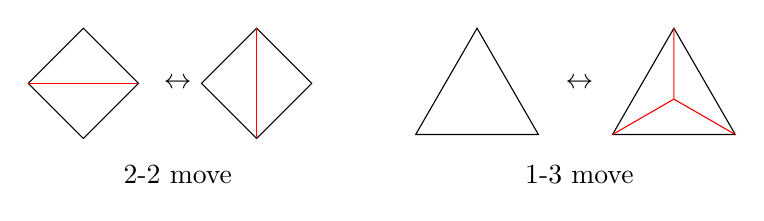
\begin{tikzpicture}
      %2-2 move
      \begin{scope}
        \coordinate (a) at (-0.7, 0);
        \coordinate (b) at (0,0.7);
        \coordinate (c) at (0.7, 0);
        \coordinate (d) at (0, -0.7);
        \draw (a)--(b)--(c)--(d)--cycle;
        \draw[red] (a)--(c);
      \end{scope}
      \node at (1.2,0) {$\leftrightarrow$};
      \begin{scope}[xshift = 2.2cm]
        \coordinate (a) at (-0.7, 0);
        \coordinate (b) at (0,0.7);
        \coordinate (c) at (0.7, 0);
        \coordinate (d) at (0, -0.7);
        \draw (a)--(b)--(c)--(d)--cycle;
        \draw[red] (b)--(d);
      \end{scope}
      \node[above] at (1.2, -1.4) {2-2 move};
      %% 3-1 move
      \begin{scope}[xshift = 5cm, yshift = -0.2cm]
      \coordinate (a) at (210:0.9cm);
      \coordinate (b) at (90:0.9cm);
      \coordinate (c) at (-30:0.9cm);
      \draw (a)--(b)--(c)--cycle;
      \end{scope}
      \node at (6.3,0) {$\leftrightarrow$};
      \begin{scope}[xshift = 7.5cm, yshift = -0.2cm]
      \coordinate (a) at (210:0.9cm);
      \coordinate (b) at (90:0.9cm);
      \coordinate (c) at (-30:0.9cm);
      \draw (a)--(b)--(c)--cycle;
      \draw[red] (0,0)--(a) (0,0)--(b) (0,0)--(c);
      \end{scope}
      \node[above] at (6.3, -1.4) {1-3 move};
    \end{tikzpicture}
  \caption{Pachner moves in dimension 2}
  \label{f:2pachner}
\end{figure}
These operations are called \emph{bistellar moves}\index{bistellar moves}, or
\emph{Pachner moves}\index{Pachner moves}. They were introduced by Pachner in
\cite{pachner}; an exposition can be found in \cite{lickorish}. They can be
easily constructed in any dimension; we show these moves in dimension 3 in
\firef{f:3pachner}, and refer the reader to the papers cited above for the
construction in arbitrary dimension.


\begin{figure}[ht]
  \centering
  \begin{tikzpicture}
    %2-3 move
    \begin{scope}
      \coordinate (a) at (0, 0);
      \coordinate (b) at (0.9,-0.2);
      \coordinate (c) at (1.3, 0.4);
      \coordinate (t) at (0.7, 1);
      \coordinate (d) at (0.8, -1);
      \path[lightyellow] (a)--(b)--(c)--(a);
      \draw (a)--(b)--(t)--cycle;
      \draw (b)--(c)--(t);
      \draw (a)--(d)--(b) (d)--(c);
      \draw[cobdash] (a)--(c);
    \end{scope}
    \node at (1.8,0) {$\leftrightarrow$};
    \begin{scope}[xshift = 2.5cm]
      \coordinate (a) at (0, 0);
      \coordinate (b) at (0.9,-0.2);
      \coordinate (c) at (1.3, 0.4);
      \coordinate (t) at (0.7, 1);
      \coordinate (d) at (0.8, -1);
      \draw (a)--(b)--(t)--cycle;
      \draw (b)--(c)--(t);
      \draw (a)--(d)--(b) (d)--(c);
      \draw[cobdash] (a)--(c);
      \draw[red] (t)--(d);
    \end{scope}
    \node[above] at (1.8, -1.8) {2-3 move};
    %% 4-1 move
    \begin{scope}[xshift = 5cm, yshift = -0.2cm]
      \coordinate (a) at (0, 0);
      \coordinate (b) at (0.9,-0.2);
      \coordinate (c) at (1.3, 0.4);
      \coordinate (t) at (0.7, 1);
      \coordinate (d) at (0.8, -1);
      \draw (a)--(b)--(t)--cycle;
      \draw (b)--(c)--(t);
      \draw[cobdash] (a)--(c);
    \end{scope}
    \node at (6.8,0) {$\leftrightarrow$};
    \begin{scope}[xshift = 7.5cm, yshift = -0.2cm]
      \coordinate (a) at (0, 0);
      \coordinate (b) at (0.9,-0.2);
      \coordinate (c) at (1.3, 0.4);
      \coordinate (t) at (0.7, 1);
      \coordinate (d) at (0.8, -1);
      \node[dotnode, red] (m) at (0.65, 0.3){};
      \draw[red] (a)--(m)--(c) (b)--(m)--(t);
      \draw (a)--(b)--(t)--cycle;
      \draw (b)--(c)--(t);
      \draw[cobdash] (a)--(c);
    \end{scope}
    \node[above] at (6.8, -1.8) {1-4 move};
  \end{tikzpicture}
  \caption{Pachner moves in dimension 3. In the second picture of the 2-3 move,
  the polyhedron is cut into 3 tetrahedra, all sharing the red edge; thus, any
  horizontal cross-section looks like the RHS of the 1-3 move in dimension 2. In
  the 1-4 move, the figure on the right is a tetrahedron cut into 4 tetrahedra,
  all sharing the center (red) vertex.}
  \label{f:3pachner}
\end{figure}

This gives us another approach to constructing invariants of manifolds (and more
generally, TQFTs): instead of using Morse functions to present a cobordism as a
composition of elementary cobordisms, we can triangulate the manifold and
construct the invariant by gluing together simplices. To check that this does
not depend on the choice of triangulation, we need to check invariance under
Pachner moves.

%%%%%%%%%%%%%%%%%%%%%%%%%%%%%%%%%%%%%%%%%%%
\section{PLCW decompositions}\label{s:PLCW}
However, for many purposes the notion of triangulation is too restrictive, and
one would like to consider more general cell decompositions --- for example,
representing a torus as the result of gluing together opposite sides of a
rectangle. In this section, we give exact definitions and results for such more
general cell decompositions, following \cite{PLCW}.

Recall that we denote by $B^k=[0,1]^k$ the $k$-ball with the canonical PL
structure; we will also use the notation $\del B^k$ and $\Int B^k= B^k - \del
B^k$ for the boundary and interior of $B^k$ respectively.


\begin{definition}\label{d:gen-cell}\index{generalized cell}
A \emph{generalized $k$-cell} in $\R^N$ is a subset $C\subset \R^N$ together
with a decomposition $C=\odot{C}\sqcup \mdot{C}$ such that $\odot{C}=\ph(\Int
B^k)$, $\mdot{C}=\ph(\del B^k)$ (and thus $C=\ph(B^k)$) for some PL map
$\ph\colon B^k\to \R^N$ which is injective on the interior of $B^k$.

In such a situation, the map $\ph$ is called a \emph{characteristic map}.
\end{definition} It is easy to show that in fact $\ph$ is determined by $C$
together with the decomposition $C=\odot{C}\sqcup \mdot{C}$, uniquely up to an
automorphism of $B^k$.

\begin{definition}\label{d:gen-complex}\index{generalized cell complex}
  A generalized cell complex (g.c.c.) is a finite collection $K$ of
  generalized cells in $\R^N$ such that
  \begin{enumerate}
    \item For any distinct $A, B$ in $K$, we have
      $$
        \odot{A}\cap \odot{B}=\varnothing
      $$
    \item For any cell $C\in K$, $\mdot{C}$ is a union of cells.
  \end{enumerate}

  The support $|K|\subset \R^N$ of a generalized cell complex $K$ is defined by
  $$
    |K|=\bigcup_{C\in K}C.
  $$

  A \emph{generalized cell decomposition}\index{generalized cell decomposition}
  of a compact polyhedron $P\subset \R^N$ is a generalized cell complex $K$ such
  that $|K|=P$.

  For a generalized cell complex $K$, we define the $k$-skeleton $K^k$ of
  $K$ as the generalized cell complex formed by all cells of dimension
  $\le k$ in $K$.
\end{definition}

This is still slightly too general; for example, this definition allows one
to form a cell decomposition by taking a rectangle and folding one of the
edges in half, gluing it to itself. To avoid that, we make the following
(recursive) definition.



\begin{definition}\label{d:PLCW}\index{PLCW complex}
  A generalized cell complex (respectively, a generalized cell
  decomposition) $K$ will be called a \emph{PLCW complex} (respectively, PLCW
  decomposition) if $\dim K=0$, or $\dim K=n>0$ and the following
  conditions hold:
  \begin{enumerate}
    \item The $(n-1)$-skeleton $K^{n-1}$ is a PLCW complex.
    \item For any $n$-cell $C\in K$, $C=\ph(B^n)$, there exists a PLCW
    decomposition $L$ of $\del B^n$ such that the restriction
    $\ph|_{\del B^n}\colon L\to K^{n-1}$ is a regular cellular map, i.e.,
    for every cell $D$ of $L$, $\ph(D)$ is a generalized cell in $K$, and
    $\ph$ is injective on $\odot{D}$.
  \end{enumerate}
\end{definition}

For $n=2$, this means the following:
\begin{itemize}
  \item The 0-skeleton is a finite collection of points (vertices) in $\R^N$.
  \item The 1-skeleton $K^1$ is a finite union of 1-cells (i.e., PL images of an
   interval), with endpoints in vertices. 1-cells are only allowed to
   intersect at endpoints; we allow two endpoints of the same interval
   to coincide.
  \item 2-cells are $k$-gons, with $k\ge 1$, and the attachment map sends each
   side of the $k$-gon to one of the 1-cells, injectively on the interior of the
   side.
\end{itemize}
In particular, we allow gluing together two sides of the same polygon, but
we do not allow, e.g., ``folding'' any side to glue it to itself.



\begin{example}\label{x:torus-plcw}
    The usual construction of a torus by gluing together opposite sides of a
    rectangle gives a PLCW decomposition of the torus, consisting of one 0-cell,
    two 1-cells, and one 2-cell.
\end{example}

Three more examples of PLCW decompositions are shown in \firef{f:plcw-examples}.

\begin{figure}[ht]
  \centering
  \begin{tikzpicture}
     %circle
    \begin{scope}
      \draw[lightyellow] (0,0) circle (0.7);
      \node[dotnode] (t) at (0,0.7) {};
    \end{scope}
    %circle
    \begin{scope}[xshift=3cm]
      \draw[lightyellow] (0,0) circle (0.7);
      \node[dotnode] (c) at (0,0) {};
      \node[dotnode] (t) at (0,0.7) {};
      \draw (c)--(t);
    \end{scope}
    %annulus
    \begin{scope}[xshift=6cm]
      \draw[lightyellow, even odd rule] (0,0) circle (0.3)
                     (0,0) circle (0.7);
      \coordinate (a1) at (0,0.3);\node[dotnode] at (a1){};
      \coordinate  (a2) at (0,0.7);\node[dotnode] at (a2){};
      \draw (a1) --  (a2) ;
    \end{scope}
  \end{tikzpicture}
  \caption{Examples of PLCW decompositions of a disk and an annulus.}
  \label{f:plcw-examples}
\end{figure}

For PLCW decompositions, we have an analog of Pachner moves. Informally,
these operations consist of erasing a $(k-1)$-disk separating two different
$k$-cells. More formally, they are defined as follows.

Let $M$ be an $n$-dimensional PL manifold together with a PLCW
decomposition $K$, and let $A=\ph(B^k)$ be a $k$-cell in $K$. Let
$L=\ph^*(K)$ be the induced PLCW decomposition of the boundary $\del
B^k=S^{k-1}$. Let $H=\{x_k=0\}$ be a hyperplane in $\R^k$; it cuts $B^k$
into two half-balls, $B_{\pm}^k$, separated by the disk $B_0^k\simeq
B^{k-1}$. Let $E=S^{k-1}\cap H$ be the equator of $S^{k-1}$. Assume that
$E$ is a union of cells of $L$. Then we can construct a subdivision of $K$
by replacing cell $A=\ph(B^k)$ by two $k$-cells $A_\pm =\ph(B_\pm^k)$ and
a $(k-1)$-cell $A_0=\ph(B_0^k)$; in other words, we ``cut'' the $k$-ball
$B^k$ into two parts by a $(k-1)$-dimensional disk. We will call such
subdivisions \emph{elementary}.

\begin{theorem}\label{t:plcw-moves}
Any two PLCW decompositions of a PL $n$-manifold $M$ can be obtained from each
other by a sequence of elementary subdivisions and their inverses.
\end{theorem}
A proof of this fact can be found in \cite{PLCW}.

For $n=2$, there are two kinds of such subdivisions:
\begin{enumerate}
  \item Subdividing a 1-cell, i.e., inserting a new vertex dividing an edge into
  two.
  \item Subdividing a 2-cell, i.e., cutting a polygon into two by a diagonal.
\end{enumerate}
Note that the word ``diagonal'' includes an arc connecting two adjacent vertices
(but does not include a loop around a vertex). These two kinds of moves are
shown in \firef{f:plcw-moves-2}.


\begin{figure}[ht]
   \centering
   % edge subdivision
   \begin{tikzpicture}
   \begin{scope}
     \coordinate (c0) at (-0.8, 0);
     \coordinate (c1) at (0.8, 0);
     \coordinate (t0) at (-1.4, 0.5);
     \coordinate (t1) at (1.4, 0.5);
     \coordinate (b0) at (-1.4, -0.5);
     \coordinate (b1) at (1.4, -0.5);
     \path[lightyellow] (t0)--(c0)--(c1)--(t1)--(t0);
     \path[lightyellow] (b0)--(c0)--(c1)--(b1)--(b0);
     \draw (t0)--(c0)--(c1)--(t1) (b0)--(c0) (c1)--(b1);
     \node[dotnode] at (c0){};
     \node[dotnode] at (c1){};
   \end{scope}
    \node at (1.75,0) {$\leftrightarrow$};
   \begin{scope}[xshift = 3.5cm]
     \coordinate (c0) at (-0.8, 0);
     \coordinate (c1) at (0.8, 0);
     \coordinate (t0) at (-1.4, 0.5);
     \coordinate (t1) at (1.4, 0.5);
     \coordinate (b0) at (-1.4, -0.5);
     \coordinate (b1) at (1.4, -0.5);
     \path[lightyellow] (t0)--(c0)--(c1)--(t1)--(t0);
     \path[lightyellow] (b0)--(c0)--(c1)--(b1)--(b0);
     \draw (t0)--(c0)--(c1)--(t1) (b0)--(c0) (c1)--(b1);
     \node[dotnode] at (c0){};
     \node[dotnode] at (c1){};
     \node[dotnode] at (0,0){};
   \end{scope}
   % polygon subdivision L
   \begin{scope}[xshift = 7cm]
     \coordinate (a0) at (0:0.7cm);
     \coordinate (a1) at (72:0.7cm);
     \coordinate (a2) at (144:0.7cm);
     \coordinate (a3) at (216:0.7cm);
     \coordinate (a4) at (288:0.7cm);
     \draw[lightyellow] (a0) --  (a1) -- (a2) -- (a3) -- (a4) -- (a0);
     \foreach \i in {0,...,4} {
       \node[dotnode] at (a\i) {};
     }
   \end{scope}
   \node at (8.2,0) {$\leftrightarrow$};
    % polygon subdivision R
   \begin{scope}[xshift = 9.2cm]
      \coordinate (a0) at (0:0.7cm);
      \coordinate (a1) at (72:0.7cm);
      \coordinate (a2) at (144:0.7cm);
      \coordinate (a3) at (216:0.7cm);
      \coordinate (a4) at (288:0.7cm);
      \draw[lightyellow] (a0) --  (a1) -- (a2) -- (a3) -- (a4) -- (a0);
      \foreach \i in {0,...,4} {
        \node[dotnode] at (a\i) {};
      }
      \draw (a0)--(a2);
    \end{scope}
  \end{tikzpicture}
  \caption{Elementary moves for $n=2$}\label{f:plcw-moves-2}
\end{figure}


A sequence of such elementary moves relating two PLCW decompositions of a disk
is shown in \firef{f:disk-subdivisions}.

\begin{figure}[ht]
  \centering
  \begin{tikzpicture}
    \begin{scope}
      \draw[lightyellow] (0,0) circle (0.6);
      \node[dotnode] (c) at (0,0) {};
      \node[dotnode] (t) at (0,0.6) {};
      \draw (c)--(t);
    \end{scope}
    \node at (1,0){$\leftrightarrow$};
    \begin{scope}[xshift = 2cm]
      \draw[lightyellow] (0,0) circle (0.6);
      \node[dotnode] (c) at (0,0) {};
      \node[dotnode] (t) at (0,0.6) {};
      \node[dotnode] (b) at (0,-0.6) {};
      \draw (c)--(t);
    \end{scope}
    \node at (3,0){$\leftrightarrow$};
    \begin{scope}[xshift = 4cm]
      \draw[lightyellow] (0,0) circle (0.6);
      \node[dotnode] (c) at (0,0) {};
      \node[dotnode] (t) at (0,0.6) {};
      \node[dotnode] (b) at (0,-0.6) {};
      \draw (b)--(t);
    \end{scope}
    \node at (5,0){$\leftrightarrow$};
    \begin{scope}[xshift = 6cm]
      \draw[lightyellow] (0,0) circle (0.6);
      \node[dotnode] (t) at (0,0.6) {};
      \node[dotnode] (b) at (0,-0.6) {};
      \draw (b)--(t);
    \end{scope}
    \node at (7,0){$\leftrightarrow$};
    \begin{scope}[xshift = 8cm]
      \draw[lightyellow] (0,0) circle (0.6);
      \node[dotnode] (t) at (0,0.6) {};
      \node[dotnode] (b) at (0,-0.6) {};
    \end{scope}
    \node at (9,0){$\leftrightarrow$};
    \begin{scope}[xshift = 10cm]
      \draw[lightyellow] (0,0) circle (0.6);
      \node[dotnode] (t) at (0,0.6) {};
    \end{scope}
  \end{tikzpicture}
  \caption{A sequence of elementary subdivisions of a disk}
  \label{f:disk-subdivisions}
\end{figure}


\clearpage
